Sign language is one of the main tools that the deaf community has both to communicate and to access information. Sign Language Recognition (SLR) has been an active research field for the last two decades \cite{camgoz2018neural}. However, each sign language has its own specific linguistic rules \cite{stokoe1980sign} and there is no direct correspondence between a sequence of words in a traditional spoken language and a sequence of signs. Therefore, an approach based on SLR, as a special case of a gesture recognition problem, is not enough to close the gap between deaf and hearing people. The problem of translating directly from sign language videos to text in the corresponding language is known as Sign Language Translation (SLT).
%\facu{Aca hablaria algo de Word vs Sentence translation, que es como se presenta en otros papers}
 Compared to other translation tasks, SLT presents unique challenges \cite{camgoz2018neural}:

\begin{itemize}

    \item The signs used and their meanings vary in different countries and even in different regions, meaning that for a model to be able to translate a specific sign language, for example, Argentinian Sign Language (LSA), it needs to be trained on data from that specific language.
    
    \item A model for SLT needs to learn not only the meaning of each sign but also the temporal dynamics and dependences between signs. Therefore, it has to be trained on videos that contain sequences of (continuous sign language or CSL). Datasets that contain isolated signs (videos containing one sign each) are not suitable for SLT.
    
    \item There are much fewer labeled sign language videos than in other domains (such as audio transcription) and there are also relatively few sign language users in the general population, which makes it difficult to find interpreters to label videos.
    
    \item Each sign is made of many components such as hand shapes, positions, movements, body poses, facial expressions, and lip movements. A model able to perform SLT should be able to use all these features.
    
    \item Typically, available videos of sign language share the same backgrounds, interpreters, or topics. This is specially true for laboratory-made datasets or, for example, videos from news channels that have a live interpreter. Models trained on this data might be biased toward these features and unable to generalize to other people or backgrounds.
    
\end{itemize}
\begin{figure}[!t]
     \centering
     \begin{subfigure}[b]{0.47\textwidth}
         \centering
         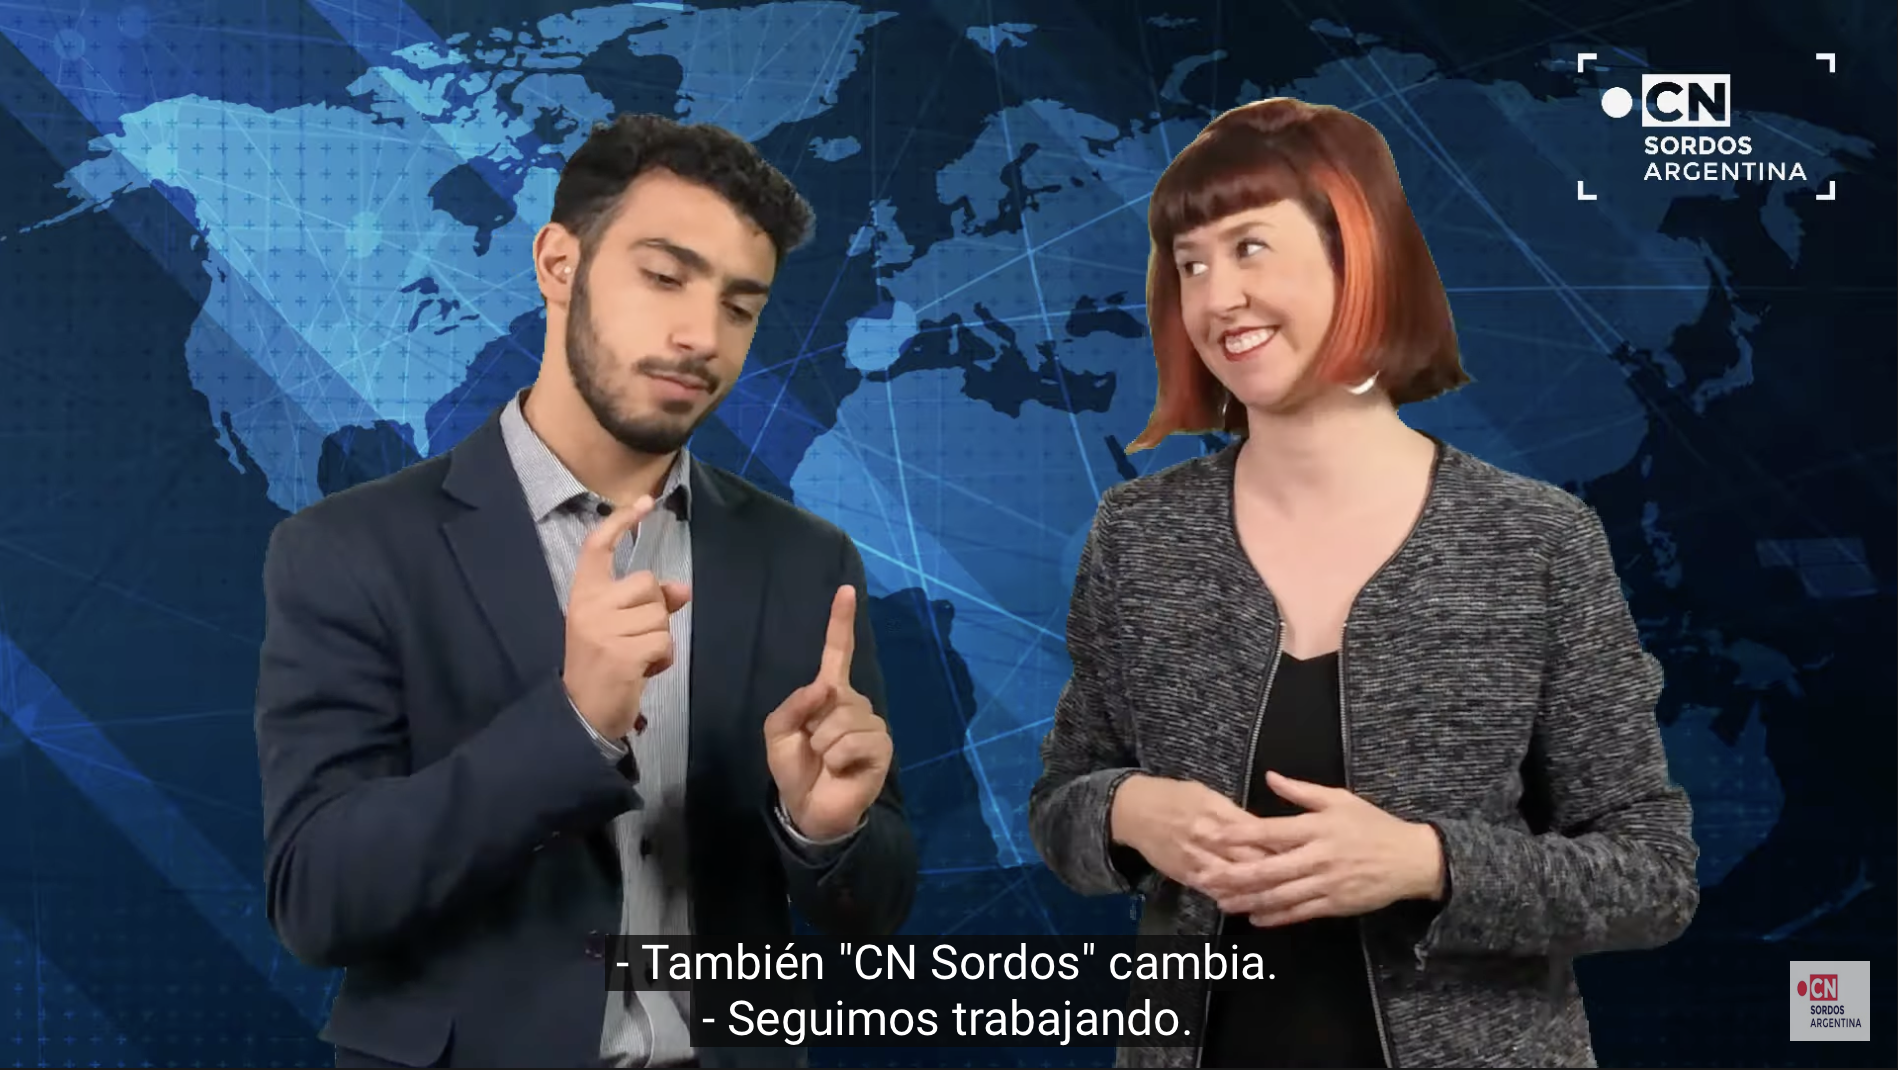
\includegraphics[width=\textwidth]{images/screenshot_resumen_semanal.png}
         \caption{"Resumen semanal"}
         \label{subfig:resumen_semanal}
     \end{subfigure}
     \hfill
     \begin{subfigure}[b]{0.47\textwidth}
         \centering
         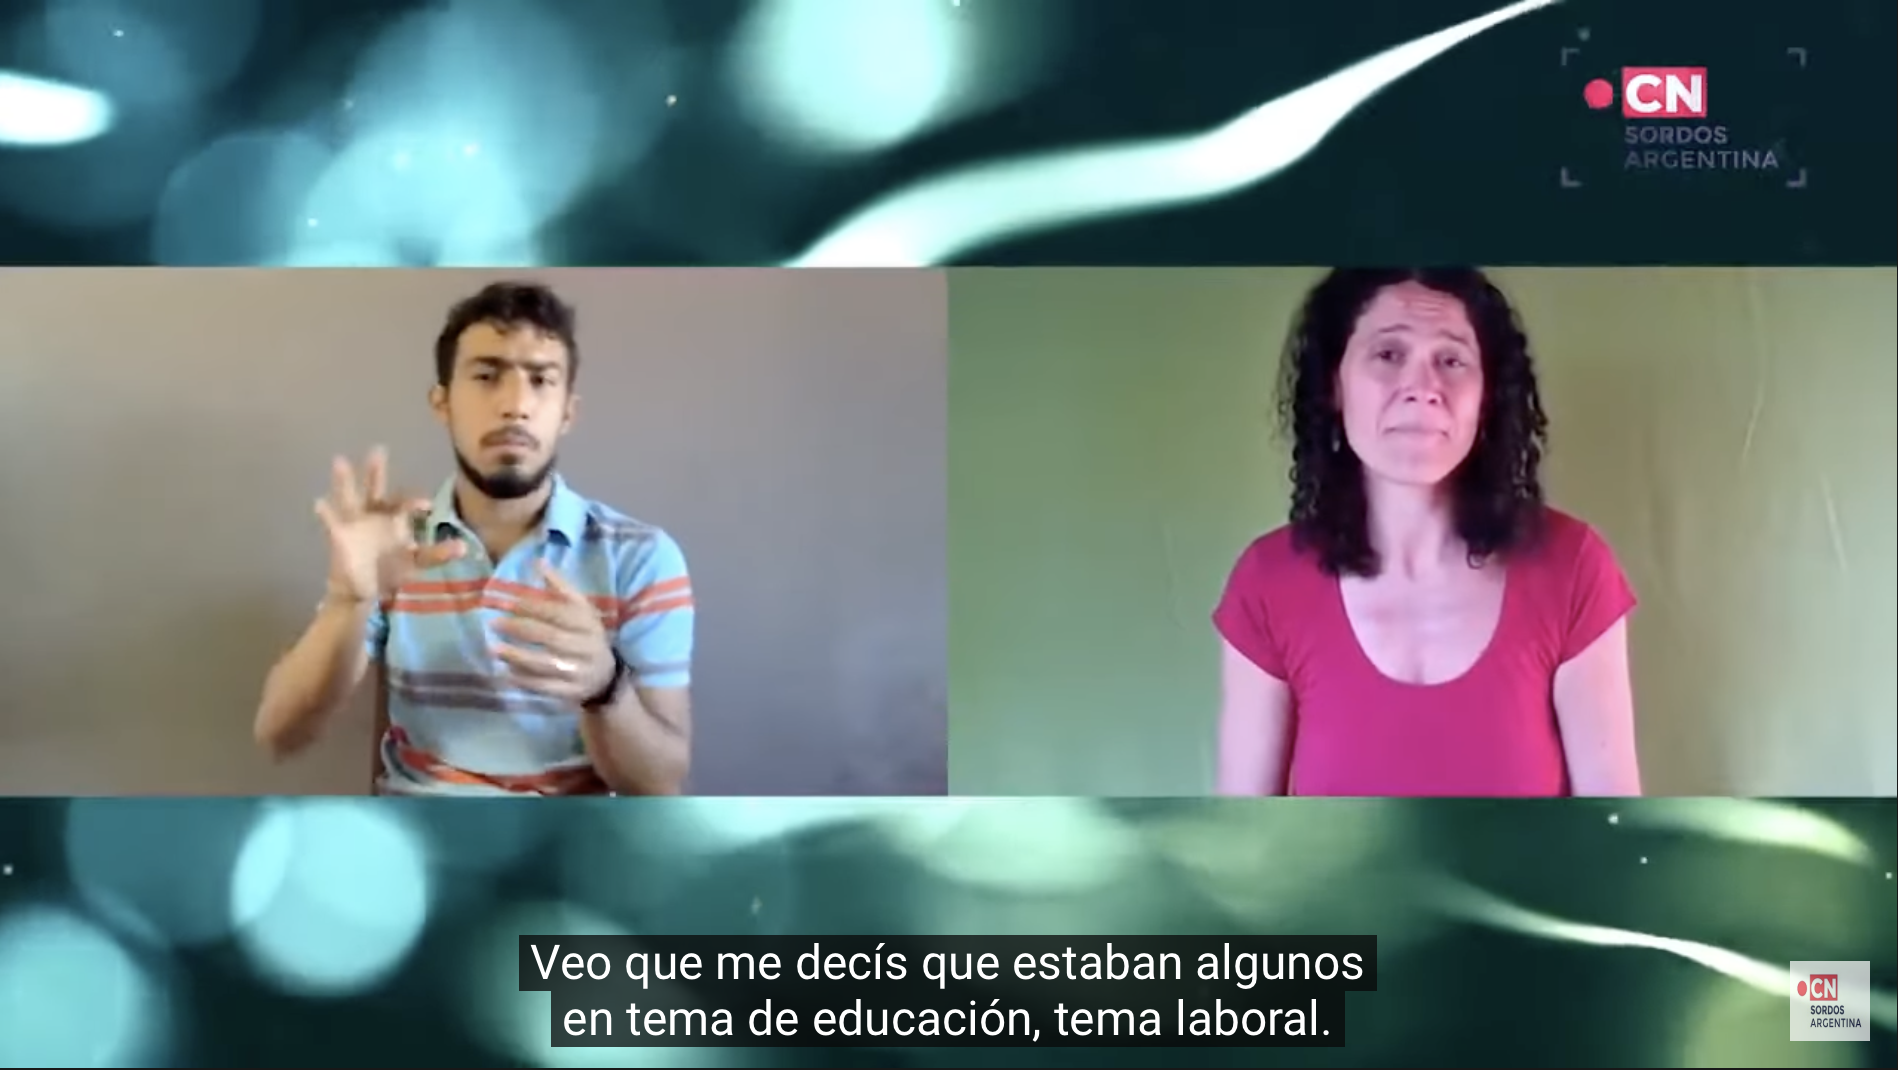
\includegraphics[width=\textwidth]{images/screenshot_ley_federal_lsa.png}
         \caption{"Ley federal LSA"}
         \label{subfig:ley_federal_lsa}
     \end{subfigure}
     \hfill
     \begin{subfigure}[b]{0.47\textwidth}
         \centering
         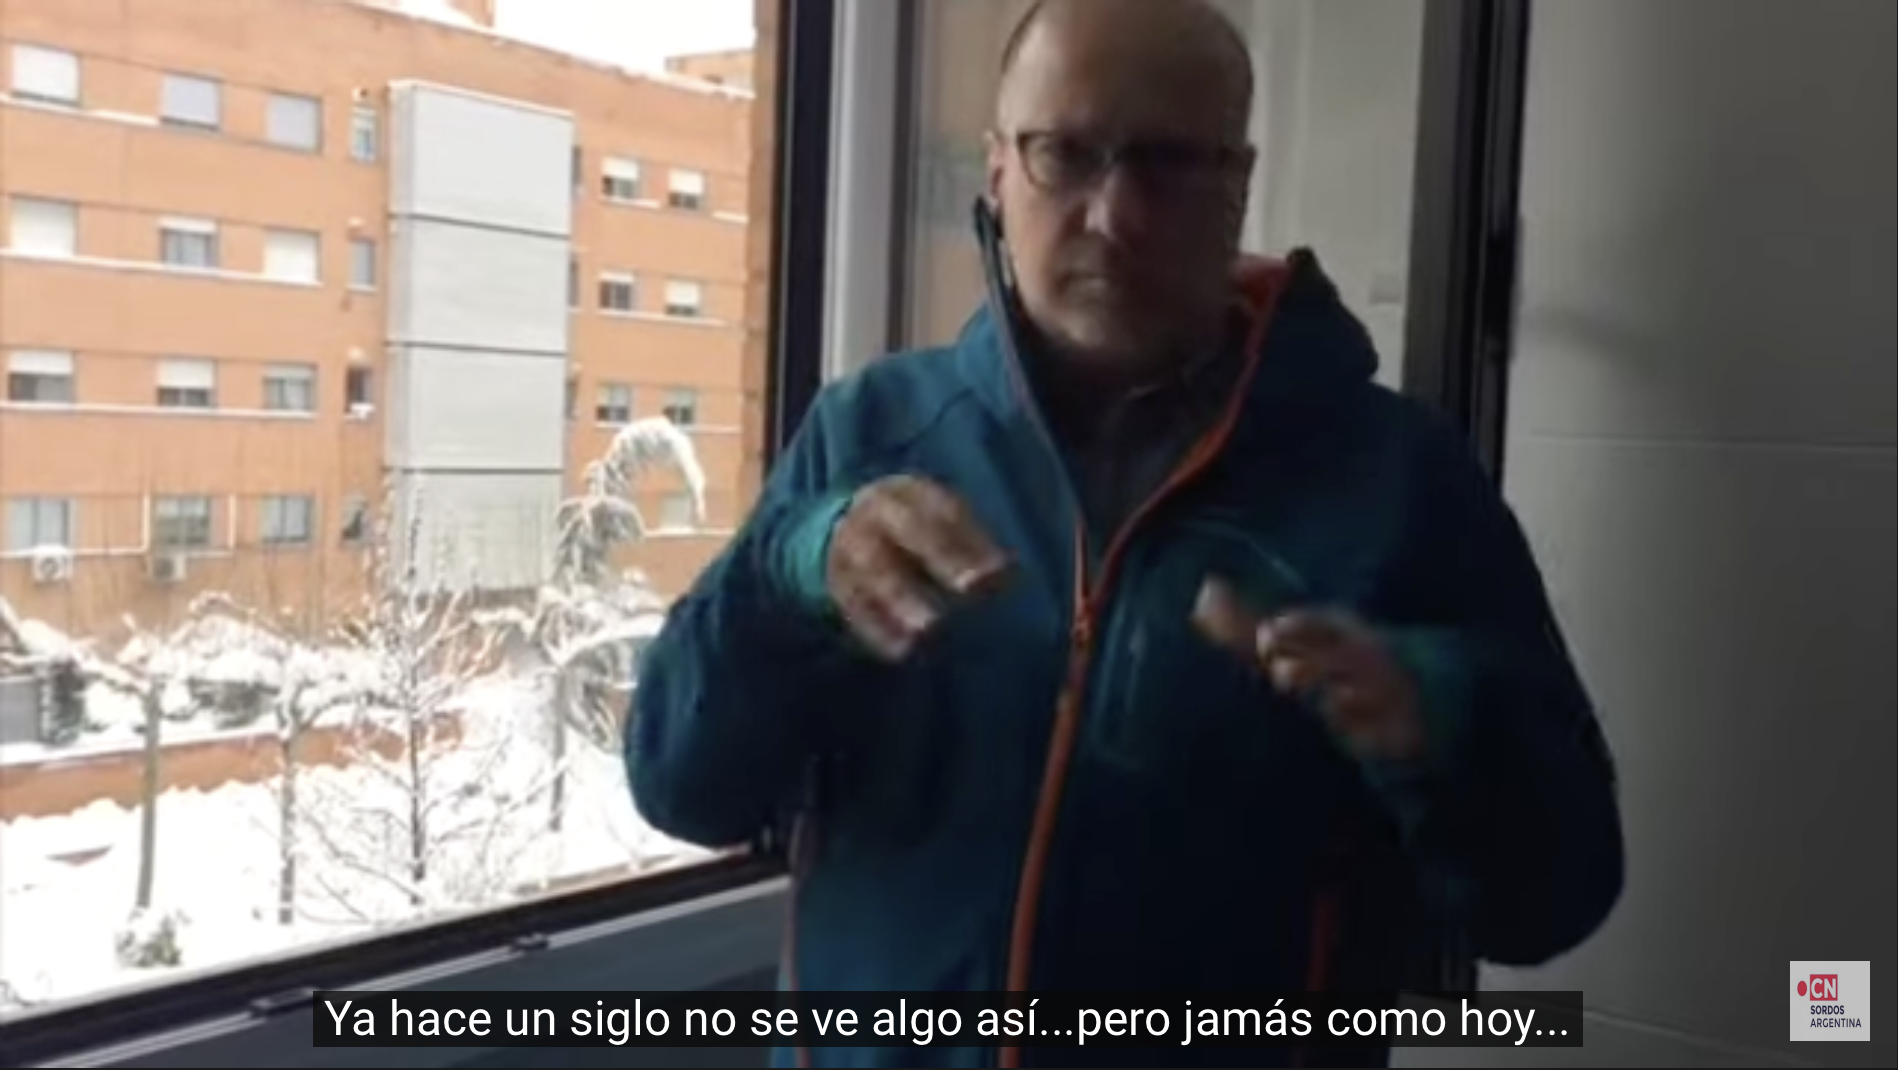
\includegraphics[width=\textwidth]{images/screenshot_ultimo_momento.png}
         \caption{"Último momento"}
         \label{subfig:ultimo_momento}
     \end{subfigure}
     \hfill
     \begin{subfigure}[b]{0.47\textwidth}
         \centering
         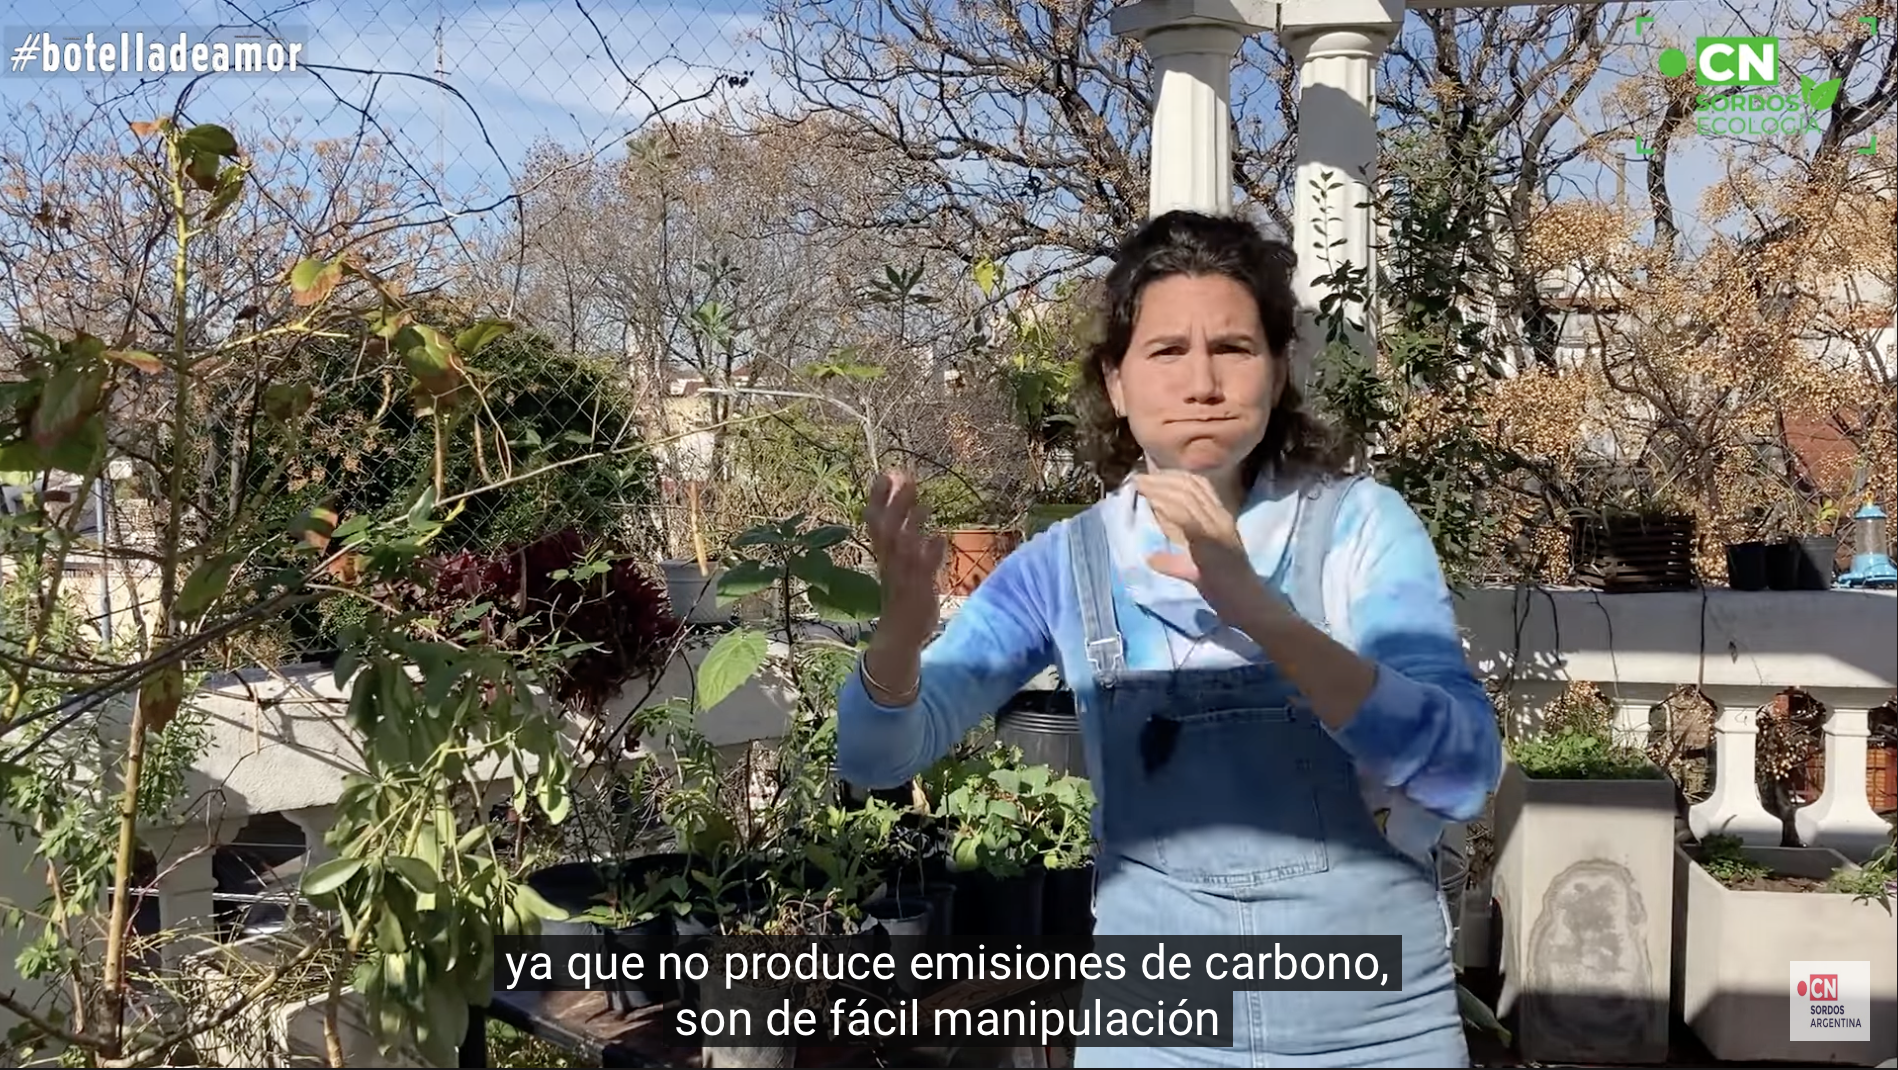
\includegraphics[width=\textwidth]{images/screenshot_cn_sordos_ecologia.png}
         \caption{"CN Sordos ecología"}
         \label{subfig:cn_sordos_ecología}
     \end{subfigure}
    \caption{Screenshots of videos from the different channel playlists.}
    \label{fig:channel_screenshots}
\end{figure}

Because of the aforementioned, a dataset that allows training models for video translation from LSA to text (and also generating LSA videos from text, altought not the focus of this work) is thought to be especially useful in order to improve the communication and inclusion of deaf people.



\subsection{Contributions}

The main contribution of this work is the presentation and analysis of \dbname: the first continuous LSA dataset. The dataset contains:

\begin{itemize}
    
    \item More than 20 hours of video extracted from CN Sordos \cite{url:cnsordos}, a YouTube channel that presents the latest news in LSA.
    
    \item The corresponding Spanish translation for the sign sentences in each video.
    
    \item The keypoints for each signer, computed using AlphaPose \cite{fang2017rmpe}.
    
    \item An estimation of the active signer in the videos where multiple people appear.

\end{itemize}

Figure \ref{fig:channel_screenshots} shows images of some of its videos. We also present a visualization tool for \dbname that allows to explore the videos present in the dataset. Finally, a model for SLT trained on this dataset is presented as a baseline. The model uses the keypoints to infer the corresponding Spanish sentence. Details of the model and its resulting metrics are described in section \ref{sec:experiments}.
